%%
%% This is file `sample-acmsmall.tex',
%% generated with the docstrip utility.
%%
%% The original source files were:
%%
%% samples.dtx  (with options: `all,journal,bibtex,acmsmall')
%% 
%% IMPORTANT NOTICE:
%% 
%% For the copyright see the source file.
%% 
%% Any modified versions of this file must be renamed
%% with new filenames distinct from sample-acmsmall.tex.
%% 
%% For distribution of the original source see the terms
%% for copying and modification in the file samples.dtx.
%% 
%% This generated file may be distributed as long as the
%% original source files, as listed above, are part of the
%% same distribution. (The sources need not necessarily be
%% in the same archive or directory.)
%%
%%
%% Commands for TeXCount
%TC:macro \cite [option:text,text]
%TC:macro \citep [option:text,text]
%TC:macro \citet [option:text,text]
%TC:envir table 0 1
%TC:envir table* 0 1
%TC:envir tabular [ignore] word
%TC:envir displaymath 0 word
%TC:envir math 0 word
%TC:envir comment 0 0
%%
%% The first command in your LaTeX source must be the \documentclass
%% command.
%%
%% For submission and review of your manuscript please change the
%% command to \documentclass[manuscript, screen, review]{acmart}.
%%
%% When submitting camera ready or to TAPS, please change the command
%% to \documentclass[sigconf]{acmart} or whichever template is required
%% for your publication.
%%
%%
\documentclass[acmsmall]{acmart}
% \documentclass[manuscript, screen, review]{acmart}

%%
%% \BibTeX command to typeset BibTeX logo in the docs
\AtBeginDocument{%
  \providecommand\BibTeX{{%
    Bib\TeX}}}

%% Rights management information.  This information is sent to you
%% when you complete the rights form.  These commands have SAMPLE
%% values in them; it is your responsibility as an author to replace
%% the commands and values with those provided to you when you
%% complete the rights form.
% \setcopyright{acmlicensed}
% \copyrightyear{2018}
% \acmYear{2018}
% \acmDOI{XXXXXXX.XXXXXXX}

%%
%% These commands are for a JOURNAL article.
% \acmJournal{JACM}
% \acmVolume{37}
% \acmNumber{4}
% \acmArticle{111}
% \acmMonth{8}

%%
%% Submission ID.
%% Use this when submitting an article to a sponsored event. You'll
%% receive a unique submission ID from the organizers
%% of the event, and this ID should be used as the parameter to this command.
%%\acmSubmissionID{123-A56-BU3}

%%
%% For managing citations, it is recommended to use bibliography
%% files in BibTeX format.
%%
%% You can then either use BibTeX with the ACM-Reference-Format style,
%% or BibLaTeX with the acmnumeric or acmauthoryear sytles, that include
%% support for advanced citation of software artefact from the
%% biblatex-software package, also separately available on CTAN.
%%
%% Look at the sample-*-biblatex.tex files for templates showcasing
%% the biblatex styles.
%%

%%
%% The majority of ACM publications use numbered citations and
%% references.  The command \citestyle{authoryear} switches to the
%% "author year" style.
%%
%% If you are preparing content for an event
%% sponsored by ACM SIGGRAPH, you must use the "author year" style of
%% citations and references.
%% Uncommenting
%% the next command will enable that style.
%%\citestyle{acmauthoryear}

% Added by me
\setcopyright{none}

%%
%% end of the preamble, start of the body of the document source.
\begin{document}

%%
%% The "title" command has an optional parameter,
%% allowing the author to define a "short title" to be used in page headers.
\title{Chiplet-Based Architectures for Scalable DNN Accelerators}

%%
%% The "author" command and its associated commands are used to define
%% the authors and their affiliations.
%% Of note is the shared affiliation of the first two authors, and the
%% "authornote" and "authornotemark" commands
%% used to denote shared contribution to the research.
% \author{Ben Trovato}
% \authornote{Both authors contributed equally to this research.}
% \email{trovato@corporation.com}
% \orcid{1234-5678-9012}
% \author{G.K.M. Tobin}
% \authornotemark[1]
% \email{webmaster@marysville-ohio.com}
% \affiliation{%
%   \institution{Institute for Clarity in Documentation}
%   \city{Dublin}
%   \state{Ohio}
%   \country{USA}
% }

% \author{Lars Th{\o}rv{\"a}ld}
% \affiliation{%
%   \institution{The Th{\o}rv{\"a}ld Group}
%   \city{Hekla}
%   \country{Iceland}}
% \email{larst@affiliation.org}

% \author{Valerie B\'eranger}
% \affiliation{%
%   \institution{Inria Paris-Rocquencourt}
%   \city{Rocquencourt}
%   \country{France}
% }

% \author{Aparna Patel}
% \affiliation{%
%  \institution{Rajiv Gandhi University}
%  \city{Doimukh}
%  \state{Arunachal Pradesh}
%  \country{India}}

% \author{Huifen Chan}
% \affiliation{%
%   \institution{Tsinghua University}
%   \city{Haidian Qu}
%   \state{Beijing Shi}
%   \country{China}}

% \author{Charles Palmer}
% \affiliation{%
%   \institution{Palmer Research Laboratories}
%   \city{San Antonio}
%   \state{Texas}
%   \country{USA}}
% \email{cpalmer@prl.com}

% \author{John Smith}
% \affiliation{%
%   \institution{The Th{\o}rv{\"a}ld Group}
%   \city{Hekla}
%   \country{Iceland}}
% \email{jsmith@affiliation.org}

% \author{Julius P. Kumquat}
% \affiliation{%
%   \institution{The Kumquat Consortium}
%   \city{New York}
%   \country{USA}}
% \email{jpkumquat@consortium.net}

\author{Darpan Gaur}
\affiliation{%
  \institution{Indian Institute of Technology, Hyderabad}
  \city{Hyderabad}
  \country{India}
}
\email{co21btech11004@iith.ac.in}

\author{Lakshay Arora}
\affiliation{%
  \institution{Indian Institute of Technology, Hyderabad}
  \city{Hyderabad}
  \country{India}
}
\email{cs24resch11006@iith.ac.in}


%%
%% By default, the full list of authors will be used in the page
%% headers. Often, this list is too long, and will overlap
%% other information printed in the page headers. This command allows
%% the author to define a more concise list
%% of authors' names for this purpose.
% \renewcommand{\shortauthors}{Trovato et al.}



%%
%% The abstract is a short summary of the work to be presented in the
%% article.
\begin{abstract}
  This paper explores the emerging role of chiplet-based architectures as a scalable and energy-efficient alternative to monolithic designs for accelerating deep learning (DL) workloads. As DL models grow in complexity, the limitations of single-die systems, in terms of rising manufacturing cost, lower fabrication yield, and lack of design reuse, have motivated the adoption of multi-chiplet solutions. Chiplet integration enables the decomposition of large accelerators into smaller, reusable components interconnected through high-bandwidth links, facilitating improved modularity and performance scalability. The paper reviews recent advancements in hardware, software, and interconnect designs for chiplet-based architectures through works including INDM \cite{INDM}, Gemini \cite{Gemini}, Florets for Chiplets \cite{florets}, and TEFLON \cite{teflon}. These works highlight the architectural, algorithmic, and thermal challenges of chiplet-based systems while demonstrating substantial gains in performance, energy efficiency, and scalability. The paper concludes by emphasizing the promise of chiplets in redefining next-generation DL accelerator design, while acknowledging ongoing challenges in mapping, communication, and system-level integration and outlining future research directions to address these issues.
\end{abstract}

%%
%% The code below is generated by the tool at http://dl.acm.org/ccs.cfm.
%% Please copy and paste the code instead of the example below.
%%
% \begin{CCSXML}
% <ccs2012>
%  <concept>
%   <concept_id>00000000.0000000.0000000</concept_id>
%   <concept_desc>Do Not Use This Code, Generate the Correct Terms for Your Paper</concept_desc>
%   <concept_significance>500</concept_significance>
%  </concept>
%  <concept>
%   <concept_id>00000000.00000000.00000000</concept_id>
%   <concept_desc>Do Not Use This Code, Generate the Correct Terms for Your Paper</concept_desc>
%   <concept_significance>300</concept_significance>
%  </concept>
%  <concept>
%   <concept_id>00000000.00000000.00000000</concept_id>
%   <concept_desc>Do Not Use This Code, Generate the Correct Terms for Your Paper</concept_desc>
%   <concept_significance>100</concept_significance>
%  </concept>
%  <concept>
%   <concept_id>00000000.00000000.00000000</concept_id>
%   <concept_desc>Do Not Use This Code, Generate the Correct Terms for Your Paper</concept_desc>
%   <concept_significance>100</concept_significance>
%  </concept>
% </ccs2012>
% \end{CCSXML}

% \ccsdesc[500]{Do Not Use This Code~Generate the Correct Terms for Your Paper}
% \ccsdesc[300]{Do Not Use This Code~Generate the Correct Terms for Your Paper}
% \ccsdesc{Do Not Use This Code~Generate the Correct Terms for Your Paper}
% \ccsdesc[100]{Do Not Use This Code~Generate the Correct Terms for Your Paper}

%%
%% Keywords. The author(s) should pick words that accurately describe
%% the work being presented. Separate the keywords with commas.
\keywords{Chiplets, dataflow mapping, 2.5D, 3D Integration, NoI/NoC, PIM, DNN}

% \received{20 February 2007}
% \received[revised]{12 March 2009}
% \received[accepted]{5 June 2009}

%%
%% This command processes the author, affiliation and title
%% information and builds the first part of the formatted document.
\maketitle

\hrulefill
\section{Introduction}

Deep neural networks (DNNs) have become foundational to modern intelligent systems, enabling breakthroughs in areas such as image classification, speech recognition, natural language processing, and autonomous control. As models grow increasingly deeper and more complex, driven by innovations like neural architecture search (NAS) and transformer-based architectures, their computational and memory demands have surged dramatically. With the slowing of Moore’s Law and the end of Dennard scaling, traditional monolithic silicon-based scaling strategies are no longer sufficient to meet the escalating performance requirements of DNN workloads.

To address these limitations, the semiconductor industry is transitioning toward chiplet-based architectures using advanced packaging technologies such as 2.5D interposers and organic substrates. These architectures decompose large chips into multiple smaller chiplets, offering advantages like improved yield, modularity, cost-efficiency, and enhanced scalability. High-bandwidth, low-latency interconnects at the package level enable effective communication between compute and memory chiplets, supporting scalable system design. Industry efforts like NVIDIA’s SIMBA \cite{Simba}, and research efforts such as NN-Baton \cite{nnBaton} and SIAM \cite{siam}, highlight the viability of chiplet-based accelerators for large-scale DNN inference.

At the same time, In-Memory Computing (IMC) has emerged as a promising approach to address the memory wall by bringing computation closer to memory. IMC architectures exploit crossbar arrays of RRAM or SRAM to perform matrix-vector operations directly within memory, achieving high parallelism and energy efficiency. However, existing IMC solutions often assume all weights are stored in a single monolithic chip, which becomes infeasible as model sizes continue to scale. Chiplet-based IMC systems offer a scalable alternative by distributing IMC tiles across multiple chiplets, allowing larger models to be supported at lower cost and improved yield. These systems can harness the compute-density advantages of IMC and the modularity of chiplet-based integration, making them ideal for next-generation DNN workloads.


Key challenges in chiplet-based DNN accelerators include:
\begin{itemize}
    \item \textbf{Communication bottlenecks:} Standard chiplet interconnects often exhibit lower bandwidth and higher latency than on-chip networks. The INDM architecture, for instance, shows that performance can be severely degraded without careful co-design of mapping strategies and interconnect topology.
    \item \textbf{Mapping complexity:} Allocating DNN layers across multiple chiplets becomes a high-dimensional optimization problem. The Gemini paper illustrates the need for intelligent mapping strategies that jointly consider data locality, load balancing, and inter-chiplet communication overheads.
    \item \textbf{Interconnect design:} As inter-chiplet dataflow becomes more critical, innovations like Floret’s dataflow-aware Network-on-Interposer (NoP) are required to balance performance, latency, and physical wiring constraints.
    \item \textbf{Thermal constraints:} High-density packaging—especially in 3D-stacked IMC systems—can lead to thermal hotspots. The TEFLON framework highlights the importance of thermally-aware NoC design and mapping strategies to maintain energy efficiency and reliability.
\end{itemize}

As DNN accelerators move toward scalable chiplet-based platforms, overcoming these challenges is essential for future progress. This paper investigates the core issues of communication, workload mapping, and thermal management in chiplet-based DNN inference systems and proposes architectural and algorithmic co-design strategies to unlock their full potential.

\section{Background}


The explosive growth in DNN model size and complexity has outpaced the capabilities of conventional monolithic hardware accelerators. Recent works have proposed chiplet-based architectures and in-memory computing paradigms that better align with DNN dataflow characteristics to address scaling challenges. This section reviews the three influential baseline architectures, SIMBA, NN-BATON, and SIAM, each exploring different dimensions of scalable DNN inference.
\subsection{SIMBA}

SIMBA  is the first chiplet-based deep learning accelerator designed to enable large-scale DNN inference with high throughput and modular scalability. The architecture (illustrated in Fig. \ref{fig:simbaArchitecture}) consists of a 2D mesh of 36 chiplets, each with 16 processing elements (PEs), a Global PE, local buffers, and a RISC-V controller. These chiplets are connected through a hierarchical interconnect—network-on-chip (NoC) within chiplets and network-on-package (NoP) across chiplets—allowing SIMBA to scale from edge devices to data-center workloads. The system achieves up to 128 TOPS with a peak efficiency of 6.1 TOPS/W.

The system uses advanced tiling strategies to efficiently map DNN computations onto SIMBA. While uniform tiling assumes equal latency and bandwidth across all compute units, this breaks down in MCM systems due to inter-chiplet communication costs. SIMBA addresses this with three optimizations: non-uniform work partitioning to balance load based on data proximity, communication-aware data placement to reduce latency by optimizing data locations, and cross-layer pipelining to increase utilization by executing different layers on separate chiplet clusters. These techniques improve performance by up to 16\% compared to baseline uniform tiling.

\begin{figure}[h]
  \centering
  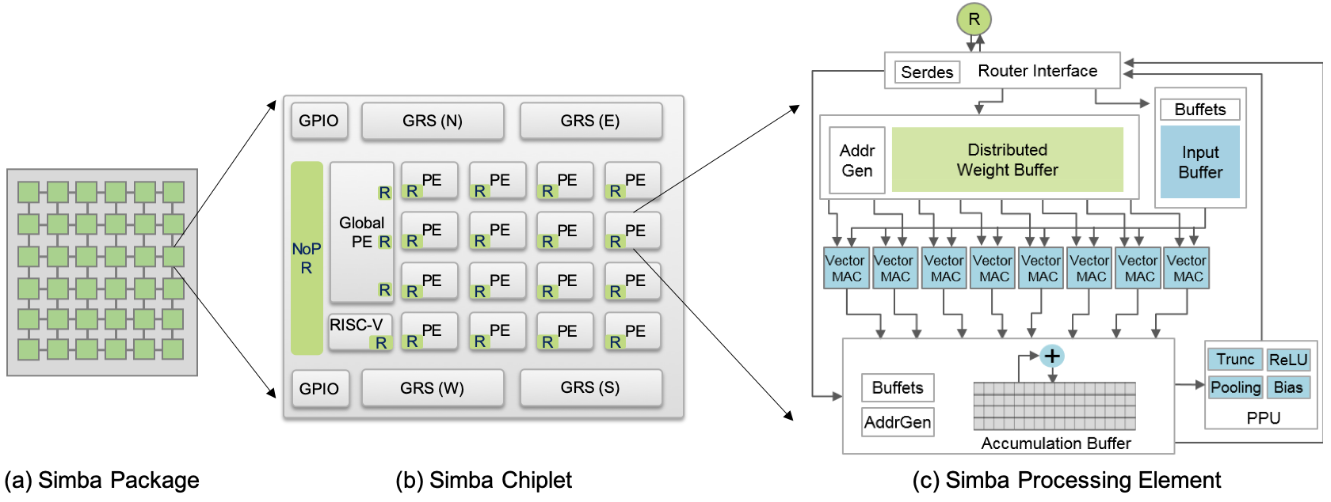
\includegraphics[width=0.8\textwidth]{figures/simbaArchitecture.png}
  \caption{Simba architecture from package to processing element (PE) \cite{Simba}}
  \label{fig:simbaArchitecture}
  
\end{figure}

\subsection{NN-BATON}

NN-BATON: Flexible System Mapping for Sparse DNN Accelerators
NN-BATON (Neural Network Balancing And Task Organization for Networked accelerators), two fundamental challenges in chiplet-based DNN accelerator design: efficient workload mapping and optimal chiplet granularity. It introduces a systematic framework to reduce inter-chip communication overhead and improve resource utilization, addressing limitations found in single-die accelerators when scaled to multichip systems.

The architecture (illustrated in Fig. \ref{fig:nnBatonArchitecture}) models three levels of parallelism—package, chiplet, and core—where cores consist of PE arrays with local buffers, grouped into chiplets with shared memory and I/O, all interconnected via a ring network. To orchestrate computation, NN-Baton adopts an output-centric dataflow model using spatial primitives for partitioning and temporal primitives for loop unrolling, maximizing data reuse. For efficient evaluation, it introduces the C3P (Critical-Capacity Critical-Position) methodology, which analytically estimates memory access overhead based on loop structure and buffer sizes, enabling fast and informed design space exploration.

Overall, NN-Baton offers a practical and analytical approach to co-designing hardware and dataflow strategies in multichip DNN accelerators, making it a foundational reference for chiplet-aware mapping and architecture exploration.


\begin{figure}[h]
  \centering
  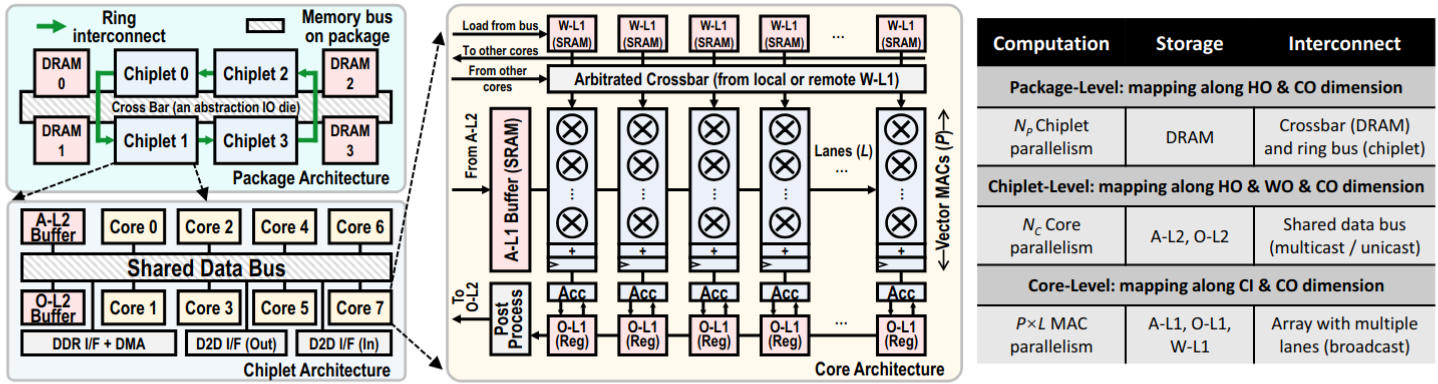
\includegraphics[width=0.8\textwidth]{figures/nnBatonArchitecture.png}
  \caption{NN-BATON: Three Level Architecture \cite{nnBaton}}
  \label{fig:nnBatonArchitecture}
\end{figure}

\subsection{SIAM}

SIAM (Scalable In-Memory Architecture for DNN Acceleration) is a first chiplet-based accelerator that uses analog in-memory computing (IMC) for matrix-vector multiplications in deep neural networks (DNNs). Unlike monolithic designs, SIAM employs a modular architecture with chiplets containing IMC cores for storing weights and performing analog Multiply-Accumulate (MAC) operations. It integrates digital interfaces, precision-tuning, and error-correction to address analog non-idealities. Each chiplet includes buffers, ADCs, pooling, and activation units, connected via on-chip NoC and Network-on-Package (NoP) for efficient chiplet communication. A global controller manages DNN layer partitioning, scheduling, and memory access. SIAM offers significant energy efficiency, up to 130× improvement over traditional GPUs like NVIDIA V100 and T4, especially for networks like ResNet-50 on ImageNet.

\begin{figure}[h]
  \centering
  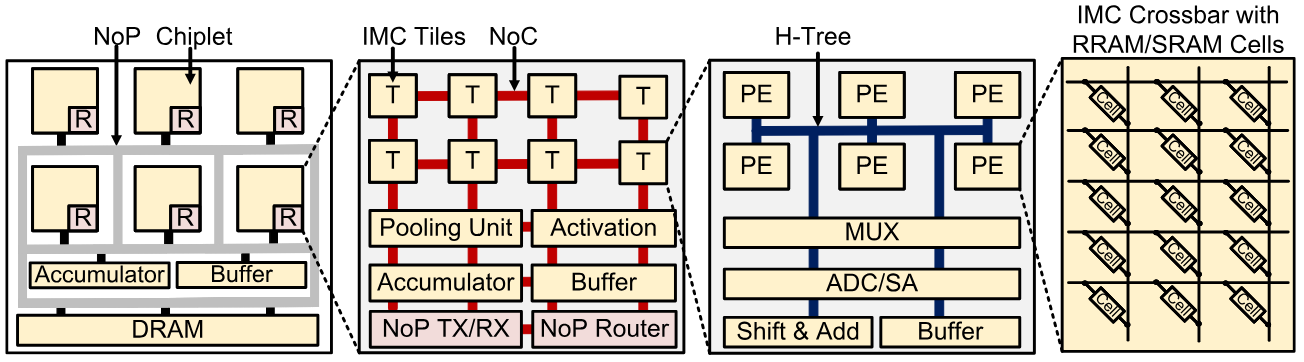
\includegraphics[width=0.8\textwidth]{figures/siamArchitecture.png}
  \caption{SIAM architecture \cite{siam}}
  \label{fig:siamArchitecture}
\end{figure}



\section{Methodology/Papers}
\subsection{INDM}
Designing deep neural network (DNN) accelerators using chiplet-based architectures introduces several critical challenges that do not exist in monolithic designs.
These include interdie communication overhead, inefficient dataflow mapping, and complex architectural partitioning.
Interdie communication significantly increases latency and energy compared to monolithic designs. Traditional mapping algorithms, optimized for single-die architectures, fail to minimize cross-chiplet data movement. 
Additionally, partitioning compute and memory resources across multiple chiplets leads to a large design space, complicating system optimization. 
INDM addresses these issues through a co-optimized framework featuring a hierarchical interconnect network, design space exploration, and interdie-aware dataflow mapping.\\

\subsubsection{Overall Architecture} 
The INDM architecture (illustrated in Fig. \ref{fig:indmArchitecture}) organizes compute dies into clusters, with every four compute dies grouped into a single cluster. Each cluster is connected internally via a dedicated IO die, which handles communication among chiplets and with external memory. Clusters are interconnected through interdie links that pass through the IO dies, forming the backbone of the system-wide interconnect. DDR memory blocks are positioned around the periphery of the package substrate to reduce I/O path lengths and latency.

Within each compute die, processing elements (PEs) share L2 buffers and are connected via a multiring on-die network. The dataflow is managed to enable the reuse of weights and activations while reducing unnecessary data transfers between chiplets. The system supports flexible parallelism at the chiplet, die, and PE levels to match the characteristics of various DNN layers.

\begin{figure}[h]
  \centering
  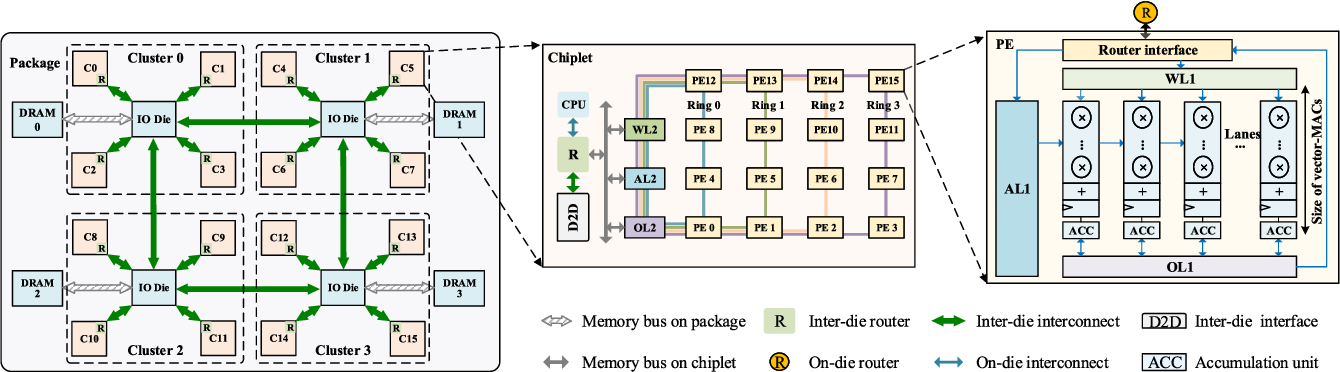
\includegraphics[width=0.8\textwidth]{figures/indmArchitecture.png}
  \caption{INDM Architecture \cite{INDM}}
  \label{fig:indmArchitecture}
\end{figure}

\subsubsection{Hierarchical Interconnect Network}
To support efficient data movement and reuse under typical DNN workloads, INDM proposes a two-level hierarchical interconnect network:
\begin{itemize}
  \item On-die communication is handled through a multiring network, which supports high-bandwidth multicast and unicast communication among PEs and shared L2 buffers. This topology reduces router complexity and facilitates efficient weight/activation distribution.
  \item Interdie communication is managed via a cluster-based topology that links compute chiplets through IO dies. Each IO die integrates DDR PHYs and controllers, minimizing the area overhead while supporting high-bandwidth DRAM access.
\end{itemize}
This network design takes advantage of DNN data reuse patterns, such as weight sharing and activation locality, to minimize traffic and balance bandwidth across the hierarchy. 
\subsubsection{Exploration of Architecture Partitioning}
To navigate the vast design space introduced by chiplet partitioning, INDM incorporates a design space exploration (DSE) framework that jointly evaluates architectural configurations and dataflow mapping strategies. This framework optimizes parameters such as the number of chiplets, buffer sizes, and interconnect topology based on target DNN workloads and hardware constraints. It balances latency, energy, and area by systematically assessing trade-offs across design points. A key feature of the framework is its latency estimation model, which offers rapid yet accurate performance predictions, significantly reducing evaluation time compared to cycle-accurate simulations. By co-optimizing architecture and mapping, the DSE framework ensures that the resulting design is scalable, energy-efficient, and well-suited to deep learning applications' communication and computation demands.

\subsection{Gemini}
As chiplet-based architectures become essential for scaling DNN accelerators in the post-Moore era, they also introduce new design complexities—particularly in mapping workloads and balancing cost, energy, and performance. Gemini addresses these challenges through a unified framework that co-explores spatial mapping and architecture design, specifically targeting large-scale DNN inference accelerators.

\subsubsection{Overall Architecture and Mapping Challenges}
Gemini is built upon a highly configurable hardware template that models realistic chiplet systems with computing and I/O chiplets connected via a mesh NoC and D2D links. This template enables various architectural configurations with tunable parameters like core counts, chiplet division (XCut, YCut), memory bandwidth, and buffer sizes. A key insight motivating Gemini is the trade-off between chiplet granularity and cost/performance efficiency: smaller chiplets improve yield but suffer from higher packaging and D2D overheads, while larger chiplets reduce interconnect cost but risk area-related yield loss.

\subsubsection{Architecture and Mapping Co-Exploration Framework}
Gemini introduces a co-optimization framework with two main engines: a Mapping Engine and a Monetary Cost (MC) Evaluator. The Mapping Engine uses a Simulated Annealing (SA) algorithm with five custom operators to explore the encoded mapping space. It iteratively improves LP mapping schemes while automatically minimizing D2D communication. Alongside, an intra-core optimizer fine-tunes tiling and loop ordering for each core.

The MC Evaluator models silicon, DRAM, and packaging costs based on architectural parameters and chiplet layouts, providing accurate cost feedback during exploration. Gemini evaluates each design using a multi-objective function combining monetary cost, energy consumption, and delay (MC·E·D), guiding the search toward practical trade-offs.


\subsection{Florets for Chiplets}
Designing chiplet-based manycore systems for concurrent CNN inference introduces unique challenges in communication efficiency, data locality, and task mapping. Traditional Network-on-Interposer (NoI) designs use multi-hop topologies like mesh and torus, which are regular and workload-agnostic. While simple to implement, these topologies perform poorly when executing diverse, large-scale CNN workloads with high contiguous inter-layer data movement. They fail to exploit the communication patterns inherent to deep learning models, resulting in excessive inter-chiplet hops, increased latency and energy consumption, and poor scalability.

\textbf{Florets} addresses these limitations by leveraging \textit{Space-Filling Curves (SFCs)} to construct a workload-aware, locality-preserving NoI topology optimized for 2.5D chiplet systems. Importantly, Florets is built atop a ReRAM-based Processing-in-Memory (PIM) architecture. By integrating ReRAM PIM within each chiplet, the design enables in-situ computation, significantly reducing data movement between compute and memory. This tight coupling of compute and memory complements the communication-efficient NoI design, enhancing both performance and energy efficiency for CNN inference workloads.


\subsubsection{Overall Architecture}
The Florets architecture organizes chiplets into multiple \textit{SFC groups}, called Florets, where each floret (or petal) cluster represents a linear contiguous path through a subset of chiplets. These florets enable efficient mapping of CNN layers to chiplets such that successive layers are placed on neighboring chiplets, reducing communication hops. Each SFC (petal) is a disjoint path with a dedicated head and tail, and inter-SFC links connect the tail of one Floret to the head of another, forming a scalable, hierarchical NoI structure.

Florets avoid uniform SFCs by assigning variable-length paths to different florets based on task requirements. A Traveling Salesman Problem (TSP)-based heuristic is used to generate low-cost SFC paths. CNN inference tasks are dynamically mapped to available chiplet sequences along these curves, ensuring minimal inter-floret transitions.



\subsubsection{Space-Filling Curve-Based NoI}
The NoI is constructed using multiple SFCs (shown in Fig. 5), each optimized for locality and minimal communication overhead. Features include:
\begin{itemize}
    \item Multiple disjoint SFCs that enable concurrent CNN execution by dividing the chiplets into separate linear paths.
    \item Workload-aware mapping aligns the CNN layer graph with the SFC paths to reduce hops.
    \item Inter-SFC links for flexibility and redundancy, enabling layers that cannot fit within one SFC to spill over with minimal latency.
\end{itemize}

\begin{figure}[h]
    \centering
    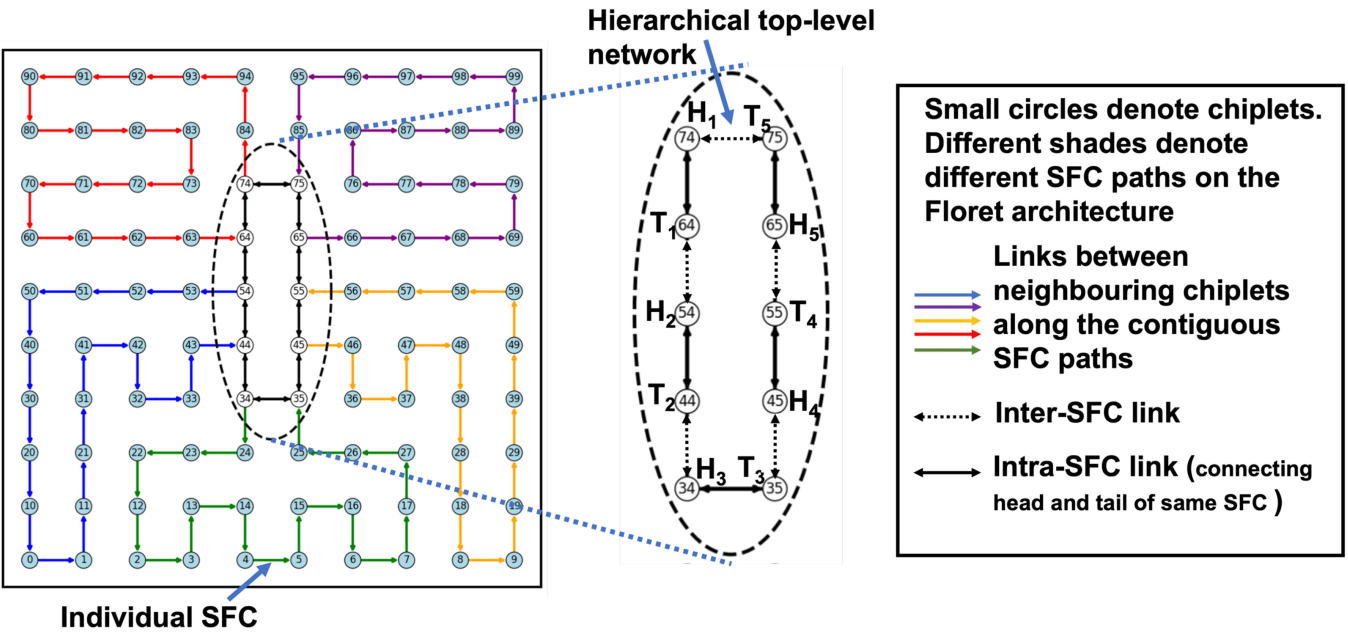
\includegraphics[width=0.8\linewidth]{figures/florets1.png}
    \caption{Illustration of the SFC-based architecture called Floret for a 100-chiplet-based system with five SFCs
on the interposer network. \cite{florets}}
    \label{fig:florets1}
\end{figure}

This design improves the spatial locality of neural layer execution and minimizes long-distance data movement, significantly enhancing throughput and energy efficiency.

\subsubsection{CNN-Aware Task Mapping Strategy}
Florets includes a dynamic layer mapping algorithm that:
\begin{itemize}
    \item Assigns CNN layers to contiguous chiplets along SFCs while balancing chiplet utilization.
    \item Supports multi-layer-per-chiplet and multi-chiplet-per-layer configurations.
    \item Minimizes inter-SFC communication by optimizing path lengths between head-tail pairs.
\end{itemize}

The algorithm ensures deadlock-free execution through sequential task allocation and considers resource reuse for future tasks. Evaluations show that Florets reduces communication latency and energy by up to \textbf{58\%} and \textbf{64\%}, while executing a diverse workload of CNN inference tasks. It also significantly reduces the fabrication costs by up to \textbf{82\%} compared to existing NoI architectures.


\subsection{TEFLON}
While SFC-based NoI designs like Florets improve communication efficiency, they do not address thermal constraints, which are critical in tightly integrated 3D manycore architectures, especially those based on ReRAM-based processing-in-memory (PIM). CNN inference on 3D systems introduces thermal hotspots that degrade performance and inference accuracy due to ReRAM conductance drift. TEFLON, an extension of Florets, proposes a thermally aware 3D NoC design methodology that optimizes for \textit{latency, energy, temperature}, and \textit{accuracy} using multi-SFC paths in a monolithic 3D (M3D) environment.

\subsubsection{Overall Architecture}
TEFLON structures its architecture around multiple 3D SFCs, where each SFC links a group of PEs across planar tiers using both horizontal and vertical links. Each SFC has a defined head and tail, and inter-SFC links enality and redundancy. TEFLON avoids stacking hivertically gh-power PEs (e.g., early CNN layers) vertically to prevent thermal hotspots. Instead, it places these layers closer to the heat sink and spreads the thermal load across tiers and planes.

Each PE integrates ReRAM crossbars and routers, and TEFLON adapts the placement of layers based on their power consumption profiles, ensuring both thermal safety and communication efficiency.

\begin{figure}[h]
    \centering
    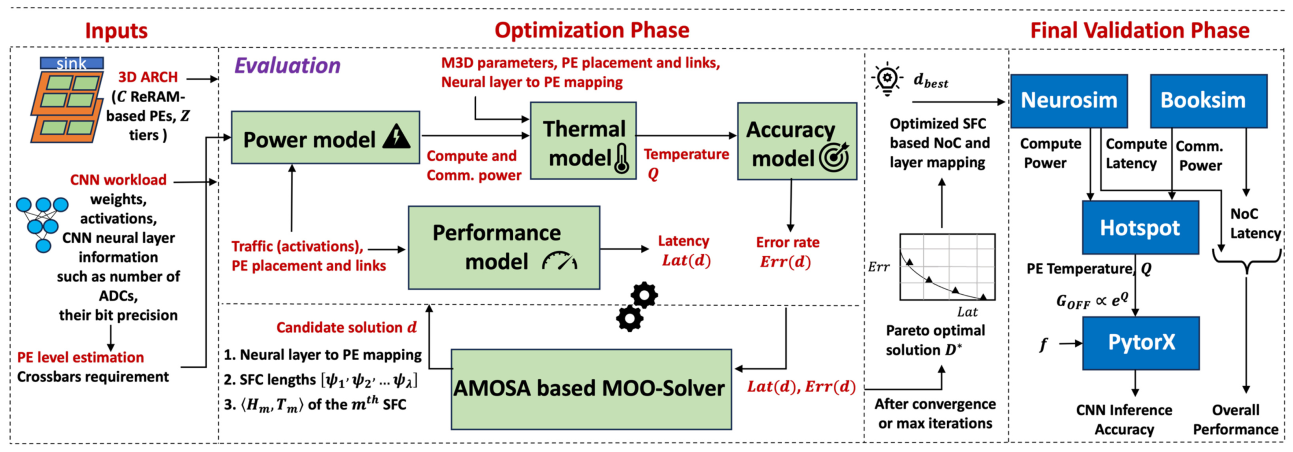
\includegraphics[width=0.8\linewidth]{figures/teflon.png}
    \caption{Overall Workflow of TEFLON \cite{teflon}}
    \label{fig:enter-label}
\end{figure}

\subsubsection{Multi-Objective SFC-Based NoC Design}
TEFLON uses a multi-objective optimization (MOO) framework to jointly minimize:
\begin{itemize}
    \item Latency (Lat) — based on activation dataflow between layers.
    \item Inference error (Err) — estimated from the thermal impact on ReRAM accuracy.
\end{itemize}

Key features include:
\begin{itemize}
    \item Dynamic PE placement along SFCs using a TSP-based heuristic.
    \item Trade-off tuning between performance and accuracy using scalarization parameters.
    \item Selection of the optimal number and lengths of SFCs to balance load, robustness, and power.
\end{itemize}

The NoC is evaluated using latency, temperature, power, and error estimation models, and Pareto-optimal configurations are selected for deployment.

\subsubsection{Thermal-Accuracy-Performance Tradeoffs}
TEFLON integrates:
\begin{itemize}
    \item HotSpot thermal modeling to prevent overheating.
    \item Weight deviation modeling in ReRAM due to thermal noise.
    \item Pruned CNN models (via coarse-to-fine pruning) to reduce power demands.
\end{itemize}

TEFLON improves inference accuracy (e.g., by up to 11\% over Florets), reduces peak chip temperature (by up to 25K), and achieves a 42--46\% reduction in Energy-Delay Product (EDP) over traditional mesh NoCs. It also introduces bypass links and router port optimization for further performance gains.


\section{Experimental Trends}
\textbf{INDM} architecture is evaluated against two leading designs: SIMBA, which uses a mesh-based interconnect, and NN-Baton, which employs ring and crossbar topologies. Both serve as baselines but struggle with scalability and interdie communication efficiency.
INDM conducts an exhaustive design space exploration under a strict 3 mm² die area constraint. Despite this, it identifies an optimal architecture with only 3.7\% EDP overhead compared to the unconstrained design. Area analysis reveals L1/L2 buffers and PE MACs as the primary components, while energy is mainly consumed by DRAM and interdie communication. As the chiplet count scales from 8 to 16 (8–128 TOPS), INDM consistently reduces latency, maintains energy efficiency, and improves overall EDP. It achieves an average 26.93\%-79.78\% latency and 26\%-73.81\% EDP reduction over SIMBA and NN-Baton, demonstrating its effectiveness across deployment scenarios.

For \textbf{Gemini}, we perform DSE on accelerators with 72, 128, and 512 TOPs to assess its architecture and mapping co-exploration capabilities. We fix compute power and vary architectural parameters like Chiplet/Core count, DRAMBW, NoCBW, D2DBW, GBUF/Core, and MAC/Core. Core arrays are arranged in near-square grids with only valid XCut/YCut values. The default setup includes TSMC 12nm, 1 GHz, organic substrate, and GRS-based D2D. We use Transformer as the main workload, with additional evaluations on ResNet-50, ResNeXt, Inception-ResNet, and PNASNet. Throughput- and latency-centric scenarios are tested using batch sizes of 64 and 1, respectively. We compare Gemini’s explored design (G-Arch, G-Map) against baselines: Simba-based (S-Arch, T-Map) and Tenstorrent-based (T-Arch, T-Map).
\begin{itemize}
  \item G-Arch vs. S-Arch: G-Arch with G-Map reduces delay by 46.8\% and energy by 28.8\% over S-Arch with T-Map, with only 14.3\% more MC. This is achieved by reducing chiplet count, increasing interconnect bandwidth, and doubling buffer capacity—minimizing D2D overhead.
  \item G-Arch vs. T-Arch: Compared to T-Arch with T-Map, Gemini improves performance by 1.74×, energy efficiency by 1.13×, and reduces MC by 40.1\%, demonstrating its effectiveness and generality.
\end{itemize}
\textbf{Floret} architecture is evaluated against state-of-the-art Network-on-Interposer (NoI) topologies such as \textit{SIMBA} and \textit{NN-Baton} in the context of 2.5D chiplet-based systems executing concurrent CNN inference tasks. These baselines are optimized for single-task performance but do not scale well under multi-task workloads due to lack of dataflow awareness. 

Floret introduces a novel space-filling curve (SFC)-based interconnect across chiplets, enabling contiguous mapping of successive CNN layers and minimizing long-range communication. The evaluation uses ReRAM-based chiplets for processing and runs multiple CNN variants including ResNet, VGG, and DenseNet. 

Compared to existing mesh-based and ring topologies, Floret consistently reduces latency by up to 58\% and energy consumption by up to 64\%, even in datacenter-scale workloads. It introduces multiple SFCs (Florets) that provide inherent redundancy, scalability, and performance isolation across tasks. It also
significantly reduces the fabrication costs by up to 82\% compared to existing NoI architectures. Experimental studies demonstrate Floret’s effectiveness in maintaining performance across increasing system sizes and concurrent inference loads, outperforming all baselines in terms of latency, energy efficiency, and chiplet utilization.

\textbf{TEFLON} is evaluated under a 3D manycore Processing-in-Memory (PIM) system with 36-, 64-, and 100-core configurations to assess its joint optimization of performance, temperature, and inference accuracy. It is benchmarked against conventional 3D mesh-based NoC architectures and the Floret-enabled SFC NoC which lacks thermal awareness.

TEFLON applies a thermally-aware, multi-SFC mapping strategy tailored for ReRAM-based CNN inference. It reduces Energy-Delay Product (EDP) by 42\%, 46\%, and 45\% on average for the 36-, 64-, and 100-PE systems respectively. Additionally, it lowers peak chip temperature by up to 25 K and improves inference accuracy by up to 11\% compared to the Floret baseline. 

TEFLON dynamically adjusts PE placement and layer mapping along the 3D SFC paths to avoid thermal hotspots while maintaining contiguity for high-activation layers. The framework uses a multi-objective optimization algorithm to jointly minimize latency and error rate under thermal constraints. It's scalable performance and thermal robustness are validated across CIFAR-10/100 workloads using diverse CNN models including \textit{VGG}, \textit{ResNet}, and \textit{DenseNet}. This robustness across varied CNN topologies highlights TEFLON's generalizability and effectiveness in real-world, high-throughput many-core inference scenarios.


\section{Challenges and Future Directions}
Chiplet-based in-memory computing offers significant potential, but several challenges remain. Inter-chiplet communication is a major bottleneck, requiring advanced, dataflow-aware interconnect designs. Efficient dataflow mapping and workload partitioning across heterogeneous chiplets remain complex and require co-optimized hardware-software strategies. Standardization of chiplet interfaces is lacking, limiting scalability and integration. Additionally, thermal management in dense 2.5D/3D IMC systems is critical, as overheating can degrade performance and accuracy—especially in analog ReRAM-based designs.

Future work should focus on holistic co-design frameworks that jointly optimize architecture, mapping, and interconnects. Thermal-aware NoC and dynamic layer placement are essential for reliability, while standardized interfaces and adaptive runtime systems can improve portability and efficiency. Advancements in compiler support and reconfigurable scheduling will also be key to unlocking the full potential of chiplet-based accelerators for DL workloads.

\section{Conclusion}
As Deep Learning models continue to scale in size and complexity, traditional monolithic accelerators face growing limitations in performance, energy efficiency, and manufacturability. This paper has examined chiplet-based architectures combined with in-memory computing as a promising alternative, offering modularity, scalability, and reduced communication overheads. By analyzing recent advances—including INDM’s hierarchical interconnects and interdie-aware dataflow mapping, Gemini’s architecture-mapping co-exploration, Floret's communication-aware NoI design, and TEFLON’s thermally optimized 3D layout—we have highlighted how thoughtful hardware-software co-design can mitigate challenges such as dataflow mapping, workload partitioning, inter-chiplet communication, and thermal constraints. Experimental results demonstrate significant improvements in latency, energy efficiency, and fabrication cost, reinforcing the potential of chiplet-based IMC for next-generation DNN accelerators. While integration and standardization remain ongoing challenges, this paradigm is well-positioned to drive the development of scalable, high-performance DL hardware systems.





%%
%% The acknowledgments section is defined using the "acks" environment
%% (and NOT an unnumbered section). This ensures the proper
%% identification of the section in the article metadata, and the
%% consistent spelling of the heading.
\begin{acks}
This paper was completed under the guidance of Dr. Rajesh Kedia, whose support and insights were essential throughout its development.
\end{acks}

%%
%% The next two lines define the bibliography style to be used, and
%% the bibliography file.
\bibliographystyle{ACM-Reference-Format}
\bibliography{sample-base}


%%
%% If your work has an appendix, this is the place to put it.
% \appendix

% \section{Write extra stuff here}



\end{document}
\endinput
%%
%% End of file `sample-acmsmall.tex'.
